Requirements engineering is a process to determine things, the desired system will consist of. This process itself consists of four stages.

\section{Elicitation}
The first faze of requirements engineering is elicitation. It's the faze of gathering information.
For us, it's these two lines:
\begin{itemize}
    %\item The student will design, implement, document and evaluate an Android-based mobile application serving as an alternative client to the current LinkedPipes ETL frontend.
    \item It will be an android-based mobile application serving as an alternative client to the current LinkedPipes ETL frontend.
    \item The application will provide pipeline and execution management and notification capabilities for multiple LinkedPipes ETL instances.
\end{itemize}

\section{Analysis}
Analysis faze is all about making sense from elicitation. It's a systematic approach to elicitation.
%One good method is describing some use cases, as shown in next table:
%\ref{tab:usecases}
%\begin{table}\centering
%	\caption[Use cases]{Use cases}\label{tab:usecases}
%	\begin{tabularx}{\textwidth}{|X|X|}
%        \hline
%        UC-1: Get overview of executions in particular server instance & Enables user to see what pipelines were executed in chronological order from specific server instance. \\ \hline
%        UC-2: Execute specific pipeline & Enables user to execute pipeline of his choice from specific server instance. \\ \hline
%        UC-3: Manage registered server instances & Enables user to register server instance in the application. Application will check, if IP is already registered or if name of the new server instance is already in use, in order to warn user about duplication or name collision that could cause chaos. It also enables user to change IP address of already registered server instance due to type error or network changes. User can also remove registered server instance. \\ \hline
%        UC-4: Manage pipelines & Enables user to manage pipelines in desired server instance. \\ \hline
%        UC-5: Re-execute pipeline from history & Enables user to quickly execute pipeline he stumbles upon while viewing history. \\ \hline
%        UC-6: Delete history & Enables user to delete items from history. \\ \hline
%        UC-7: View execution history & Enables user to view execution history of all the instances at the same time. \\ \hline
%        UC-8: View pipelines & Enables user to view pipelines from all the server instances. \\ \hline
%        UC-9: Be notified on execution finish & User has the option to be notified about execution completion. \\ \hline      
%	\end{tabularx}
%\end{table}
\subsection{Use cases}
One good method of achieving this is by describing some use cases. Each use case is something that user expects from the system. We will also create scenarios for the non trivial ones. Scenario is an array of tasks user should do in order to go through the use case.

\subsubsection*{UC-1: Get overview of executions in particular server instance}
Enables user to see what pipelines were executed in chronological order from specific server instance.
\subsubsection*{UC-2: Execute specific pipeline}
Enables user to execute pipeline of his choice from specific server instance.
\subsubsection*{UC-3: Manage registered server instances}
Enables user to register server instance in the application. Application will check, if IP is already registered or if name of the new server instance is already in use, in order to warn user about duplication or name collision that could cause chaos. It also enables user to change IP address of already registered server instance due to type error or network changes. User can also remove registered server instance.
\subsubsection*{UC-4: Manage pipelines}
Enables user to manage pipelines in desired server instance.
\subsubsection*{UC-5: Re-execute pipeline from history}
Enables user to quickly execute pipeline he stumbles upon while viewing history.
\subsubsection*{UC-6: Delete history}
Enables user to delete items from history.
\subsubsection*{UC-7: View execution history}
Enables user to view execution history of all the instances at the same time.
\subsubsection*{UC-8: View pipelines}
Enables user to view pipelines from all the server instances.
\subsubsection*{UC-9: Be notified on execution finish}
User has the option to be notified about execution completion.

%\subsubsection*{Diagram}
\begin{figure}\centering
	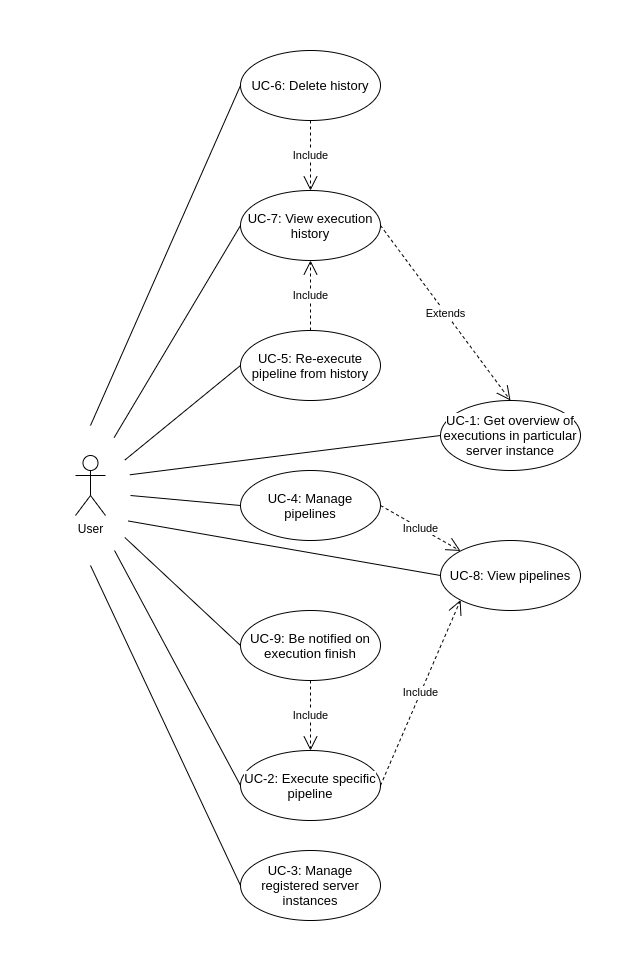
\includegraphics[width=0.9\textwidth]{pics/bc-uc.png}
	\caption[Use cases]{Diagram consisting of use cases}\label{fig:uc}
\end{figure}

%For better perspective, here is a diagram of all these use cases: \ref{fig:uc}

\subsection{Scenarios}
Now we can create some scenarios for the user.

\subsubsection*{SC-1.1: Get overview of executions in particular server instance}
User opens execution history screen and selects what server instance executions he wants to see.
\subsubsection*{SC-2.1: Execute specific pipeline}
User opens pipeline list screen. He then finds the desired pipeline and execute it. Optional: After opening the pipeline screen, user can filter pipelines by the server instance.
\subsubsection*{SC-3.1: Change IP address or name of registered server instance}
User opens settings screen, selects the desired server instance for edit. He then changes the IP address and saves changes.
\subsubsection*{SC-3.2: Register server instance}
User opens settings screen, tells the application he wants to register new server instance and proceeds to enter server instance info and saves it.
\subsubsection*{SC-3.3: Delete registered server instance}
User opens settings screen, views registered server instances and tells the application what server instance he wants to delete, followed by confirmation.
\subsubsection*{SC-4.1: Create pipeline}
User opens pipeline list screen. Then he tells the application he wants to create a new pipeline. He chooses a server instance to which the pipeline will be saved and the screen for editing pipeline will be launched and the user can design a new pipeline here. When he is finished, he will save the pipeline.
\subsubsection*{SC-4.2: Edit pipeline}
User opens pipeline list screen. He then finds the desired pipeline and tells the application he wants to edit it. The screen for editing pipeline will be launched with the selected pipeline loaded so the user can make and save changes here. Optional: After opening the pipeline screen, user can filter pipelines by the server instance.
\subsubsection*{SC-4.3: Delete pipeline}
User opens pipeline list screen. He then finds the desired pipeline and tells the application he wants to delete it. This request is followed by confirmation. Optional: After opening the pipeline screen, user can filter pipelines by the server instance.
\subsubsection*{SC-5.1: Re-execute pipeline from history}
User opens execution history screen. He finds a pipeline and realize he wants to execute it now, so he tells that to the application. Optional: After opening the execution history screen, he can selects what server instance executions he wants to see.
\subsubsection*{SC-6.1: Delete history}
User opens execution history screen. He finds a record and realize he for some reason doesn't want this record in history anymore, so he tells that to the application. Optional: After opening the execution history screen, he can selects what server instance executions he wants to see.
\subsubsection*{SC-9.1: Be notified}
User executes specific pipeline, just like in SC-2.1. Application will notify user about the execution completion. This will happen only if it is allowed in settings.

\section{Specification}
The goal of this section is to produce a structured document consisting of functional requirements.
\subsection*{F-1.0: Settings screen}
Application must have a separate screen for settings. It can be seen in scenarios SC-3.1, SC-3.2, SC-3.3.
\subsection*{F-2.1: View server instance}
List of server instances will be visible from settings screen. It can be seen in scenarios SC-3.1, SC-3.3.
\subsection*{F-2.2: Add server instance}
User must be able to add server instance. It can be seen in scenarios SC-3.2.
\subsection*{F-2.3: Edit server instance}
User must be able to edit already added server instance. It can be seen in scenarios SC-3.1.
\subsection*{F-2.4: Delete server instance}
User must be able to delete already added server instance. Confirmation will be required. It can be seen in scenarios SC-3.3.
\subsection*{F-2.5: Deactivate server instance}
User can deactivate server instance in settings instead of deleting it, so it is possible to activate it again later easily. App will not communicate with deactivated server instances.
\subsection*{F-3.1: Notification after finish}
Application shell create notification on pipeline finish. It can be seen in scenarios SC-9.1.
\subsection*{F-3.2: Notifications in settings}
There will be switch in settings to toggle notifications. It can be seen in scenarios SC-9.1.
\subsection*{F-4.0: Pipeline list screen}
Application must have a separate screen for working with pipelines. Which pipelines will be visible there depends on F-4.7. It can be seen in scenarios SC-2.1, SC-4.1, SC-4.2, SC-4.3.
\subsection*{F-4.1: View pipelines}
List of pipelines will be visible from pipeline list screen. Which pipelines will be visible depends on F-4.7. It can be seen in scenarios SC-2.1, SC-4.2, SC-4.3.
\subsection*{F-4.2: Edit pipeline screen}
Application must have a screen for editing pipelines. It can be seen in scenarios SC-4.1, SC-4.2.
\subsection*{F-4.3: Create pipelines}
User must be able to start an empty edit pipeline screen (F-4.2) from the pipeline list screen (F-4.0). It can be seen in scenarios SC-4.1.
\subsection*{F-4.4: Edit existing pipelines}
User must be able to edit selected pipeline by starting the edit pipeline screen (F-4.2) with the selected activity loaded. It can be seen in scenarios SC-4.2.
\subsection*{F-4.5: Delete pipelines}
User must be able to delete a pipeline of his choice. It can be seen in scenarios SC-4.3.
\subsection*{F-4.6: Execute pipeline}
User must be able to execute selected pipeline. It can be seen in scenarios SC-2.1.
\subsection*{F-4.7: Source for visible pipelines}
User must be able to choose, if he wants to see pipelines from all instances, or just a specific one. It can be seen in scenarios SC-2.1, SC-4.2, SC-4.3.
\subsection*{F-5.0: Execution history screen}
Application must have a separate screen for execution history. History of which server instance will be visible depends on F-5.4 It can be seen in scenarios SC-1.1, SC-5.1, SC-6.1.
\subsection*{F-5.1: View execution history}
List of executions will be visible from the execution history screen. History of which server instance will be visible depends on F-5.4 It can be seen in scenarios SC-1.1, SC-5.1, SC-6.1.
\subsection*{F-5.2: Delete items from history}
User must be able to delete specific item from execution history. Confirmation will be required. It can be seen in scenarios SC-6.1.
\subsection*{F-5.3: Re-execute pipelines from history}
There must be an option to re-execute pipeline from the execution history screen. This action will also make a new record in execution history. It can be seen in scenarios SC-5.1.
\subsection*{F-5.4: Source of visible history}
User must be able to choose, if he wants to see history of all instances, or just a specific one. It can be seen in scenarios SC-1.1, SC-5.1, SC-6.1.
\subsection*{F-6.1: Night mode}
User can have an option in settings to use light or dark theme, or use system default theme (Android 10 and newer).
\subsection*{F-2.6: Ping server}
User can test if the server address is correct

\section{Validation}
In this stage I went through all of previous stages, corrected some typos. I gave everything a second look, to verify everything is somehow testable.